% -*- mode: LaTeX; TeX-PDF-mode: t; -*- 
% LaTeX path to the root directory of the current project
% from the directory in which this file resides
% and path to econtexPaths which defines the rest of the paths like \FigDir
\providecommand{\econtexRoot}{}\renewcommand{\econtexRoot}{.}
\providecommand{\econtexPaths}{}\renewcommand{\econtexPaths}{econtexPaths}
% -*- mode: LaTeX; TeX-PDF-mode: t; -*- 
% The \commands below are required to allow sharing of the same base code via Github between TeXLive on a local machine and Overleaf (which is a proxy for "a standard distribution of LaTeX").  This is an ugly solution to the requirement that custom LaTeX packages be accessible, and that Overleaf prohibits symbolic links
\providecommand{\packages}{\econtexRoot/Resources/texmf-local/tex/latex}
\providecommand{\econtex}{\packages/econtex}
\providecommand{\econark}{\econtexRoot/Resources/texmf-local/tex/latex/econark}
\providecommand{\econtexSetup}{\econtexRoot/Resources/texmf-local/tex/latex/econtexSetup}
\providecommand{\econarkSetup}{\econtexRoot/Resources/texmf-local/tex/latex/econarkSetup}
\providecommand{\econtexShortcuts}{\econtexRoot/Resources/texmf-local/tex/latex/econtexShortcuts}
\providecommand{\econtexBibMake}{\econtexRoot/Resources/texmf-local/tex/latex/econtexBibMake}
\providecommand{\econtexBibStyle}{\econtexRoot/Resources/texmf-local/bibtex/bst/econtex}
\providecommand{\econtexBib}{economics}
\providecommand{\notes}{\econtexRoot/Resources/texmf-local/tex/latex/handout}
\providecommand{\handoutSetup}{\econtexRoot/Resources/texmf-local/tex/latex/handoutSetup}
\providecommand{\handoutShortcuts}{\econtexRoot/Resources/texmf-local/tex/latex/handoutShortcuts}
\providecommand{\handoutBibMake}{\econtexRoot/Resources/texmf-local/tex/latex/handoutBibMake}
\providecommand{\handoutBibStyle}{\econtexRoot/Resources/texmf-local/bibtex/bst/handout}

\providecommand{\FigDir}{\econtexRoot/Figures}
\providecommand{\CodeDir}{\econtexRoot/Code}
\providecommand{\DataDir}{\econtexRoot/Data}
\providecommand{\SlideDir}{\econtexRoot/Slides}
\providecommand{\TableDir}{\econtexRoot/Tables}
\providecommand{\ApndxDir}{\econtexRoot/Appendices}

\providecommand{\ResourcesDir}{\econtexRoot/Resources}
\providecommand{\rootFromOut}{..} % APFach back to root directory from output-directory
\providecommand{\LaTeXGenerated}{\econtexRoot/LaTeX} % Put generated files in subdirectory
\providecommand{\econtexPaths}{\econtexRoot/Resources/econtexPaths}
\providecommand{\LaTeXInputs}{\econtexRoot/Resources/LaTeXInputs}
\providecommand{\LtxDir}{LaTeX/}
\providecommand{\EqDir}{\econtexRoot/Equations} % Put generated files in subdirectory

\providecommand{\titlepagecustom}{\LaTeXInputs/titlepagecustom}


\documentclass[\econtexRoot/HAFiscal]{subfiles}
\onlyinsubfile{\providecommand{\econtexRoot}}
\onlyinsubfile{\renewcommand{\econtexRoot}{..}}
\onlyinsubfile{\externaldocument{\econtexRoot/HAFiscal}} % Get xrefs -- esp to apndx -- from main file; only works if main file has already been compiled

\begin{document}

\FloatBarrier
\hypertarget{comparing-fiscal-stimulus-policies}{}\par\section{Comparing fiscal stimulus policies}
\notinsubfile{\label{sec:comparing}}

In this section, we present our results where we compare three policies to provide fiscal stimulus in our calibrated model. The policies we compare are a means-tested stimulus check, an extension of unemployment benefits, and a payroll tax cut. Each policy is implemented at the start of a recession, and we compare results both with and without aggregate demand effects being active during the recession. First, we present impulse responses of aggregate income and consumption after the implementation of each policy. Then we compare the policies in terms of their cumulative multipliers and in terms of their effect on a welfare measure that we introduce. Finally, based on these comparisons, we can rank the three policies. 

\hypertarget{impulse-responses}{}\par\subsection{Impulse responses}
\notinsubfile{\label{sec:IRFs}}

The impulse responses that we present for each stimulus policy are constructed as follows: 
\begin{itemize} 
\item A recession hits in quarter one. 
\item We compute the subsequent path for the economy without any policy introduced in response to the recession. 
\item We also compute the subsequent path for the economy with a given policy introduced at the onset of the recession in quarter one. 
\item The impulse responses we present are then the \textit{difference} between these two paths for the economy and show the effect of a policy relative to a case where no policy was implemented.
\item The solid lines show these impulse responses for an economy where the aggregate demand effects described in section~\ref{sec:ADeffects} are not active, and the dashed lines show impulse responses for an economy where the aggregate demand effects are active during the recession. 
\item Red lines refer to aggregate labor and transfer income, and blue lines refer to consumption. 
\end{itemize}

Note that all graphs show the average response of income and consumption for recessions of different length.
Specifically, we simulate recessions lasting from only one quarter up to 20 quarters.
We then take the sum of the results across all recession lengths weighted by the probability of this recession length occurring (given our assumption of an average recession length of six quarters).

\subsubsection{Stimulus check} 



\begin{figure}[htb]
	\centering
	\begin{subfigure}[b]{.33\linewidth}
		\centering
		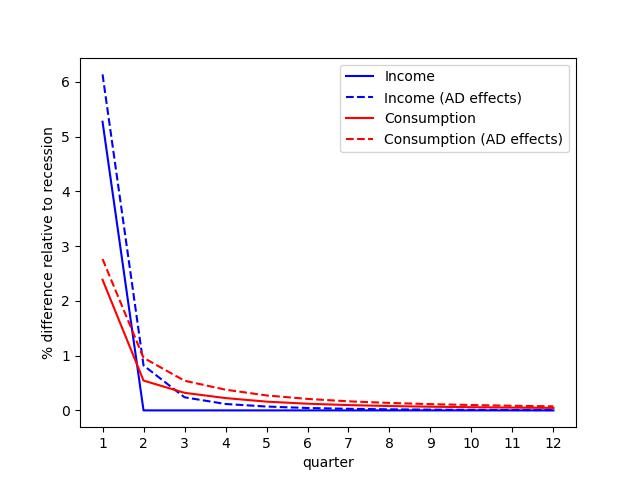
\includegraphics[width=\linewidth]{\econtexRoot/Code/HA-Models/FromPandemicCode/Figures/recession_Check_relrecession}
		\caption{stimulus check - IRF}
		\notinsubfile{\label{fig:recessioncheckrelrecession}}
	\end{subfigure}%
	\begin{subfigure}[b]{.33\linewidth}
		\centering
		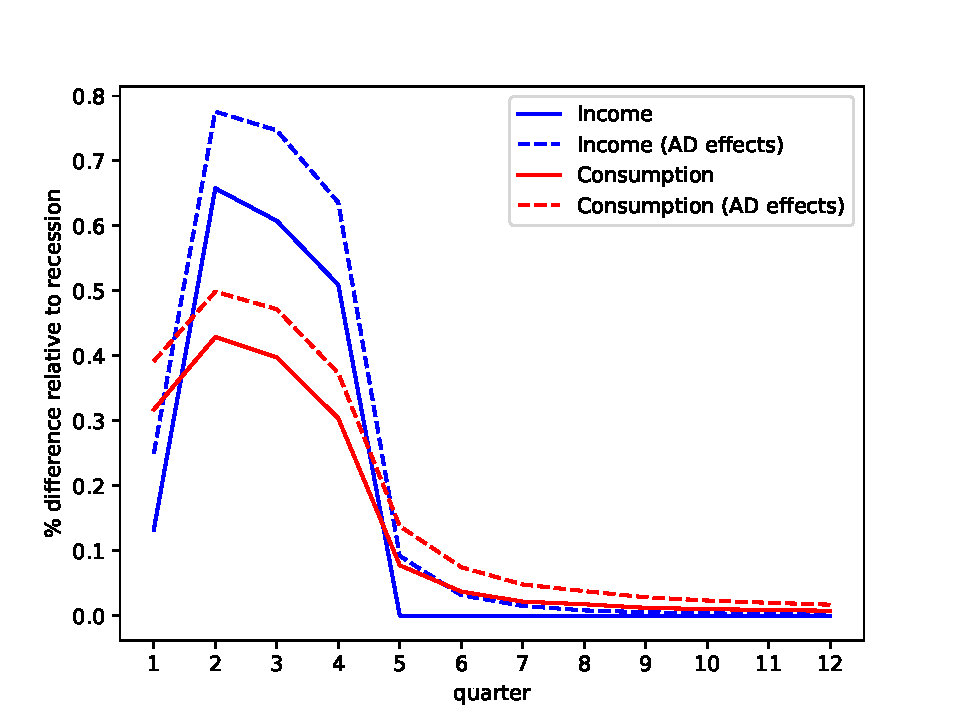
\includegraphics[width=\linewidth]{Code/HA-Models/FromPandemicCode/Figures/recession_UI_relrecession}
		\caption{UI extension - IRF}
		\notinsubfile{\label{fig:recessionuirelrecession}}
	\end{subfigure}%
	\begin{subfigure}[b]{.33\linewidth}
		\centering
		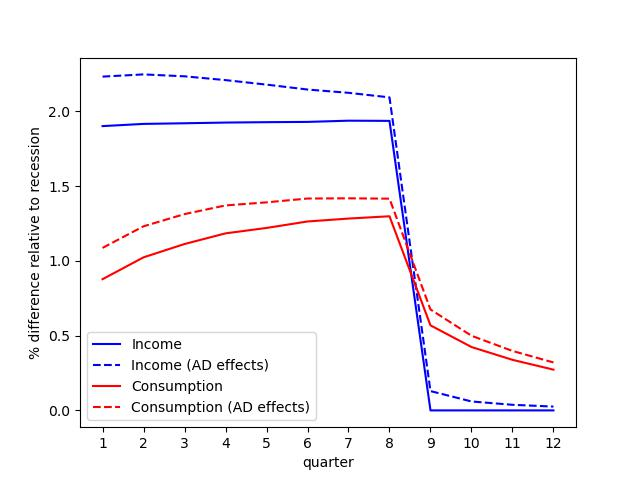
\includegraphics[width=\linewidth]{Code/HA-Models/FromPandemicCode/Figures/recession_taxcut_relrecession}
		\caption{payroll tax cut - IRF}
		\notinsubfile{\label{fig:recessiontaxcutrelrecession}}
	\end{subfigure}\\
		\begin{subfigure}[b]{.33\linewidth}
		\centering
		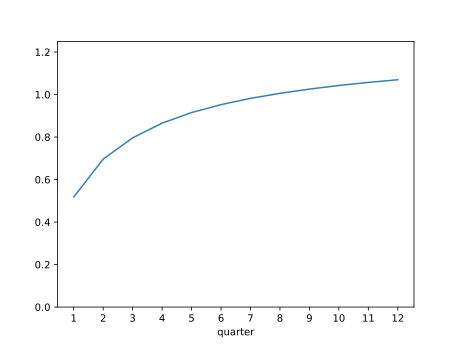
\includegraphics[width=\linewidth]{\econtexRoot/Code/HA-Models/FromPandemicCode/Figures/Cummulative_multiplier_Check}
		\caption{stimulus check - cumulative multiplier}
		\notinsubfile{\label{fig:recessioncheckrelrecession_Mult}}
	\end{subfigure}%
	\begin{subfigure}[b]{.33\linewidth}
		\centering
		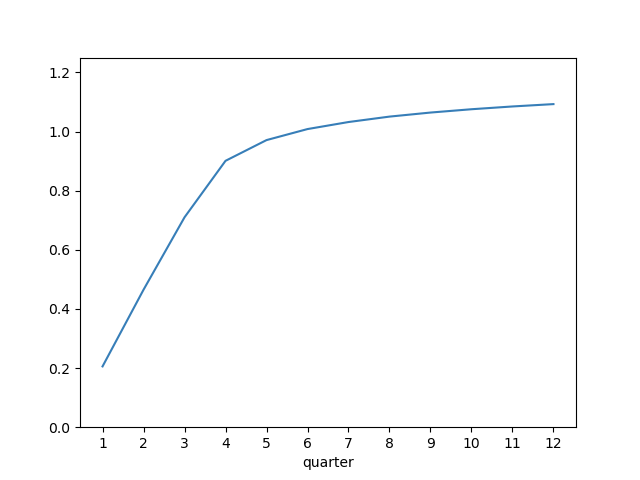
\includegraphics[width=\linewidth]{Code/HA-Models/FromPandemicCode/Figures/Cummulative_multiplier_UI}
		\caption{UI extension - cumulative multiplier}
		\notinsubfile{\label{fig:recessionuirelrecession_Mult}}
	\end{subfigure}%
	\begin{subfigure}[b]{.33\linewidth}
		\centering
		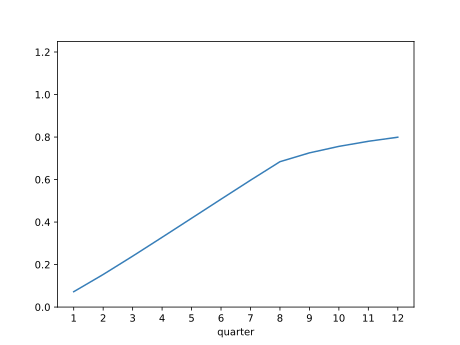
\includegraphics[width=\linewidth]{Code/HA-Models/FromPandemicCode/Figures/Cummulative_multiplier_TaxCut}
		\caption{payroll tax cut - cumulative multiplier}
		\notinsubfile{\label{fig:recessiontaxcutrelrecession_Mult}}
	\end{subfigure}
	\caption{Impulse responses of aggregate income and consumption to policy shocks during recessions with and without aggregate demand effects as well as cumulative multipliers as a function of the horizon for the three policies.
{\label{fig:Policyrelrecession}}}
	\parbox{16cm}{\small \vspace{.15cm} \textbf{Note}: For the cumulative multiplier plots, policies are implemented during a recession with aggregate demand effects active.\normalsize}
\end{figure}



Figure \ref{fig:recessioncheckrelrecession} shows the impulse response of income and consumption when stimulus checks are issued in the first quarter of a recession.
In the model without a multiplier, the stimulus checks account for 5 percent of the first quarter's income.
In the following quarters, there are no further stimulus payments, and income remains the same as it would have been without the stimulus check policy.
Consumption is about 2.5 percent higher in the first quarter, which includes the splurge response to the stimulus check.
Consumption then drops to less than 1 percent above the counterfactual, and the remainder of the stimulus check money is then spent over the next few years.
In the model with aggregate demand effects, income in the first quarter is 6 percent higher than the counterfactual, as the extra spending feeds into higher incomes.
Consumption in this model jumps to a higher level than without aggregate demand effects and comes down more slowly as the feedback effects from consumption to income dampen the speed with which income---and hence the splurge---return to zero.
After a couple of years, when the recession is most likely over and aggregate demand effects are no longer in place, income is close to where it would be without the stimulus check policy, although consumption remains somewhat elevated.

\subsubsection{UI extension}


The impulse responses in Figure \ref{fig:recessionuirelrecession} show the response to a policy that extends unemployment benefits from 6 months to 12 months for a period of a year.
In the model without aggregate demand effects, the path for income now depends on the number of consumers who receive the extended unemployment benefits.
These consumers are those who have been unemployed for between 6 and 12 months.
In the first quarter of the recession, the newly unemployed receive unemployment benefits regardless of whether they are extended or not.
Therefore, it is in the second and third quarters, when the effects of the recession on long-term unemployment start to materialize, that the extended UI payments ramp up, amounting to an aggregate increase in quarterly income by 0.7 percent.
By the fifth quarter, the policy is no longer in effect, and income from extended unemployment goes to zero.
Consumption in the first quarter jumps by more than income (by 0.3 percent), prompted by both the increase in expected income and the reduced need for precautionary saving given the extended insurance.
In the model without aggregate demand effects, consumption is only a little above the counterfactual by the time the policy is over.
In the model with aggregate demand effects, there is an extra boost to income of about the same size in the first and second quarters.
As this extra aggregate demand induced income goes to employed consumers, more of it is saved, and consumption remains elevated several quarters beyond the end of the policy.

\subsubsection{Payroll tax cut}



The final impulse response graph, Figure \ref{fig:recessiontaxcutrelrecession}, shows the impulse response for a payroll tax cut that persists for two years (eight quarters).
In the model without aggregate demand effects, income rises by close to 2 percent as the take-home pay for employed consumers goes up.
After the two-year period, income drops back to where it would have been without the payroll tax cut.
Consumption jumps close to 1 percent in response to the tax cut.
Over the period in which the tax cut is in effect, consumption rises somewhat as the stock of precautionary savings goes up.
Following the drop in income, consumption drops sharply because of the splurge and then decreases over time as consumers spend out the savings they built up over the period the tax cut was in effect.
In the model with aggregate demand effects, income rises by about 2.3 percent above the counterfactual and then declines steadily as the probability that the recession remains active---and hence the aggregate demand effects in place---goes down over time.
Following the end of the policy, the savings stock in the model with aggregate demand effects is high, and consumption remains significantly elevated through the period shown.

\hypertarget{multipliers}{}\par\subsection{Multipliers}
\notinsubfile{\label{sec:multipliers}}

In this section, we compare the fiscal multipliers across the three stimulus policies.
Specifically, we employ the cumulative multiplier, which captures the ratio between the net present value (NPV) of stimulated consumption up to horizon $t$ and the full-horizon NPV of the cost of the policy.
We thus define the cumulative multiplier up to horizon $t$ as
\begin{equation}
	\label{eqn:cumMultiplier}
  M(t) = \frac{NPV(t,\Delta C)}{NPV (\infty,\Delta G)},
\end{equation}
where $\Delta C$ is the additional aggregate consumption spending up to time $t$ in the policy scenario relative to the baseline and $\Delta G$ is the total government expenditure caused by the policy.
The NPV of a variable $X_t$ is given by 
$NPV(t,X) = \sum_{s=0}^{t} \left( \prod_{i=1}^{s} \frac{1}{R_i} \right) X_s$.

The multiplier hence captures the amount of induced consumption at different horizons relative to the total (i.e.
full-horizon) cost of the policies.\footnote{In the case that there is no aggregate demand effect, these multipliers converge to 1 as $t$ goes to infinity.}


The second row in Figure \ref{fig:Policyrelrecession} plots the cumulative multipliers at different horizons, and table \ref{tab:Multiplier} shows the 10y-horizon multiplier for each policy.
The stimulus check, which is paid out in quarter one, exhibits the largest multiplier on impact.
About 50 percent of the total policy expenditure is immediately spent by consumers.
After two years, and because of the aggregate demand effects, consumption has increased cumulatively by more than the cost of the stimulus check.
Over time, the policy reaches a total multiplier of 1.199.
Without AD effects the policy only generates a multiplier of 0.854.
The last two rows in table \ref{tab:Multiplier} show the expected share of the policy expenditures and stimulated consumption that occurs during a recession.
For the stimulus check all of the policy expenditures occur in the first quarter and thus with certainty during the recession.
However, since induced consumption also takes place during later periods at which time the recession may have already ended, the share of stimulated consumption during the recession is lower at 75\%.

Since spending for the UI policy is spread out over four quarters (and peaks in quarters two to three), the multiplier in the first quarter is considerably lower than in the case of the stimulus check.
However, the UI extension policy is targeted in the sense that it provides additional income only to those consumers who have large MPCs, because of unemployment.
Also, over the medium-term UI extension expenditures are more likely to induce consumption spending during the recession compared to the check stimulus, see the last row in table \ref{tab:Multiplier}.
This is because UI extension expenditures affect agents who spend the additional income relatively quickly once it reaches them.
Therefore, the cumulative mulitiplier of the UI extension exceeds that of the stimulus check after about one year.


\begin{table}[t]
  \center
  \begin{tabular}{@{}lccc@{}} 
\toprule 
& Tax Cut    & UI extension    & Stimulus check    \\  \midrule 
Long-run Multiplier (AD effect) &0.968  & 1.180  & 1.228     \\ 
Long-run Multiplier (1st round AD effect only) &0.000  & 0.000  & 0.000     \\ 
Share of policy expenditure during recession &45.0\%  & 72.0\%  & 100.0 \%    \\ 
\end{tabular}  

  \caption{Multipliers as well as the share of the policy expenditure and consumption stimulus occurring during the recession}
  \parbox{16cm}{\small \vspace{.15cm} \textbf{Note}: Policies are implemented during a recession with or without the aggregate demand effect active. The row "1st round AD effect only" captures the direct consumption impact of the policies and the additional boost to consumption resulting from the aggregate demand effect acting on the direct consumption impact. It does not include higher-round aggregate demand effects materializing on aggregate demand effects acting on indirectly stimulated consumption.\normalsize}
  \notinsubfile{\label{tab:Multiplier}}
\end{table}

The payroll tax cut has the lowest multiplier irrespective of the considered horizon.
A multiplier of close to 1 is reached only after 10 years with AD effects.
These relatively small numbers reflect that policy spending lasts for a long time and is thus more likely to occur after the recession has ended.
Moreover, only employed consumers, often with relatively low MPCs, benefit directly from the payroll tax cut.
Therefore, the policy is poorly targeted if the goal is to provide short-term stimulus.

Table \ref{tab:Multiplier} contains an additional (middle) row with results for an economy where we only consider a ``first-round'' aggregate demand effect.
To understand these values note that the policies initially increase the income of consumers directly, which leads to a boost in consumption.
As a consequence, this boost triggers an aggregate demand effect which increases the income of everyone and in turn leads to an additional boost to consumption.
We refer to the sum of this initial and the indirect boost to consumption as the first-round AD effect.
However, the AD effect continues as the indirect boost to consumption triggers another round of income increases which further boost consumption and so on.
One might argue that these higher-order rounds of the AD effect are not likely to be anticipated by consumers.
Since higher-order consumption boosts only materialize if consumers anticipate them and act accordingly, the overall increase in consumption might turn out to be smaller than suggested by the full AD effect.
As shown in the middle row of the table, the multipliers are smaller when excluding higher-order rounds.
Nevertheless, the ranking of the policies remains unchanged.


\hypertarget{welfare}{}\par\subsection{Welfare}
\notinsubfile{\label{sec:welfare}}

In this section, we look at the welfare implications of each stimulus policy.
To do so, we need a way to aggregate welfare in our model with individual utility functions.
In our model, some households consume much less than other households, and a social planner with equal weights on each household could significantly increase welfare through redistribution across households even in normal times.
We are interested in the benefit of carrying out fiscal policies in a recession, so we do not want our results to reflect the benefits of redistribution inherent in our model in normal times.

Our welfare measure weights the felicity of a household at time $t$ by the inverse of the marginal utility of the same household in a counterfactual simulation in which neither the recession occurred nor the fiscal policy was implemented, discounted by the real interest rate.\footnote{Discounting at the real interest rate accounts for the fact that a redistributive policy over time will require borrowing or lending at the real interest rate.
The preference discount factors of households would appear in both the numerator and the denominator---the utility and marginal utility---and therefore cancel and do not play a role in our welfare measure.} This weighting scheme means that in normal times the marginal benefit or cost to a social planner of moving a dollar of consumption from one household at one time period to another household at the same or a different time period is zero.
Hence, in normal times, any re-distributive policy has zero marginal benefit.
However, in a recession when the average marginal utility is higher than in normal times, there can be welfare benefits to government borrowing to allow households to consume more during the recession.

As with all social welfare measures, ours is not without ethical issues.
We have chosen our welfare measure over one with equal weights because an equal-weights measure would be increasing with the size of any redistributive policy.\footnote{Using a version of an equal-weights measure results in an even greater welfare benefit to extended unemployment insurance---see the previously distributed draft of this paper, \cite{carroll2023welfare}.
However, because the size of the extended unemployment benefits policy is much larger in a recession compared to normal times, while the size of the other two policies does not change significantly in a recession, this equal-weights measure almost mechanically favored the extended unemployment benefits policy.}
However, similar to Negishi weights, our welfare measure gives greater weight to households that are well off.\footnote{Negishi weights have been used in the climate literature as a way to separate the welfare benefits of climate mitigation policies from broader questions about global income redistribution.
Our problem of separating the welfare benefits of recession mitigation policies from income redistribution in normal times is similar, but complicated by our incomplete markets setup.
With complete markets, under which there is no potential benefit to redistributing consumption across time for any individual household, our measure is identical to Negishi weights.}
Furthermore, our welfare measure distinguishes between households that would have suffered unemployment in normal times and households that are made unemployed as a result of the recession—--giving the latter a higher weight in the social welfare function.

Let $\mathbf{c}_{it,\textit{normal}}$ be the consumption---inclusive of the splurge---of household $i$ at time $t$ in the baseline simulation with no recession and no fiscal policy.
The (undiscounted) marginal utility of an extra unit of consumption for this household in this time period is $ u'(\mathbf{c}_{it,\textit{normal}})$.


Let $\mathbf{c}_{it,\textit{policy},Rec,AD}$ be the consumption of the same household under the fiscal policy, $\textit{policy}$, possibly a recession, $Rec \in \{0,1\}$, and in an economy with or without aggregate demand effects, $AD \in \{0,1\}$.\footnote{In the simulations, household $i$ experiences the same permanent and transitory shock sequence, but in the recession simulation some households experience unemployment during periods in which the same household is employed in the baseline simulation.}

We also denote the net present value of the government expenditures of the policy as $NPV(\textit{policy},Rec,AD)$.
With this notation, we can now define the welfare bang for the buck of a policy as:

\begin{equation}\begin{gathered}\begin{aligned} \label{welfare_def6}
	\mathcal{W}(\text{policy},Rec,AD) =\frac{1}{NPV(\text{policy},Rec,AD)}\sum_{i=1}^{N} \sum_{t=0}^{\infty} \frac{1}{R^t} \frac{u(\mathbf{c}_{it,\textit{policy},Rec,AD}) - u(\mathbf{c}_{it,\textit{none},Rec,AD})}{ u'(\mathbf{c}_{it,\textit{normal}})} ,
\end{aligned}\end{gathered}\end{equation}
% We can consider displaying the equation below instead which looks slightly nicer?
%\begin{equation}\begin{gathered}\begin{aligned} \label{welfare_def6_alt}
%	\mathcal{W}(\text{policy},Rec,AD) =\frac{\sum_{i=1}^{N} \sum_{t=0}^{\infty} \frac{1}{R^t} \frac{u(\mathbf{c}_{it,\textit{policy},Rec,AD}) - u(\mathbf{c}_{it,\textit{none},Rec,AD})}{ u'(\mathbf{c}_{it,\textit{normal}})}}{NPV(\text{policy},Rec,AD)},
%\end{aligned}\end{gathered}\end{equation}

In normal times, this welfare measure will be exactly equal to one for any small-scale fiscal expansion.
To see this, note that the numerator,  $u(\mathbf{c}_{it,\textit{policy},0,0}) - u(\mathbf{c}_{it,\textit{none},0,0})$, is equal to the change in consumption multiplied by the marginal utility in normal times.
As the total change in consumption is equal to the net present value of the policy, which we divide by, the total welfare measure is equal to one.
Note that for large increases in consumption, this measure may be less than one because the utility function is concave.

\begin{table}[ht] 
	\center
	\begin{tabular}{@{}lccc@{}} 
\toprule 
                          & Stimulus check      & UI extension    & Tax cut    \\  \midrule 
$\mathcal{W}(\text{policy}, Rec=0, AD=0)$ & 1.00  & 0.85  & 1.00     \\ 
$\mathcal{W}(\text{policy}, Rec=1, AD=0)$ & 1.03  & 1.83  & 0.98     \\ 
$\mathcal{W}(\text{policy}, Rec=1, AD=1)$ & 1.40  & 2.15  & 1.12     \\ \bottomrule 
\end{tabular}  

	\caption{Welfare measures, calculated for policies implemented both out of and in a recession with and without aggregate demand effects}
	\notinsubfile{\label{welfare6}}
\end{table}

Table \ref{welfare6} shows the welfare measure for each policy as defined by equation \eqref{welfare_def6}.
The top row of the table shows the welfare measure for implementing each policy in normal times.
For marginal policies, this is equal to one by definition.
Indeed, the value for both the stimulus check and the tax cut policy is very close to one.
However, the welfare measure for the extended unemployment policy in normal times is noticeably less than one.
This is because, although this policy is smaller in absolute size than the other policies, its consumption effects are concentrated on a small number of households that remain unemployed long enough to receive the extended benefits.
For these households, the effect on consumption is large enough such that the non linearity of the consumption function leads to smaller welfare benefit than the marginal utility of consumption would otherwise imply.

The second row of table \ref{welfare6} shows the welfare benefit of each policy in a recession without any aggregate demand effects.
Again, the stimulus check and tax cut policies have measures that are close to one---pulling forward consumption has little welfare benefit for the average household because the average marginal utility of consumption is only a little higher than in normal times.
By contrast, the policy sees benefits of 1.8 dollars for every dollar spent on extended UI benefits during a recession.
This is because many of the households who are unemployed for many quarters in the recession would have never been unemployed, or quickly reemployed, in normal times and hence their marginal utility of consumption is much higher in the recession than in normal times.

The third row of the table shows the welfare measure for each policy in a recession in the version of the model with aggregate demand effects during the recession.
The payroll tax cut now has a noticeable benefit, as some of the tax cut gets spent during the recession, resulting in higher incomes for all consumers.
However, the tax cut is received over a period of two years, and much of the relief may be after the recession---and hence the aggregate demand effect---is over.
Furthermore, because the payroll tax cut goes only to employed consumers who have relatively lower MPCs, the spending out of this stimulus will be further delayed, possibly beyond the period of the recession.
By contrast, the stimulus check is received in the first period of the recession and goes to both employed and unemployed consumers.
The earlier arrival and higher MPCs of the stimulus check recipients mean more of the stimulus is spent during the recession, leading to greater aggregate demand effects, higher income, and higher welfare.
The extended UI arrives, on average, slightly later than the stimulus check.
However, the recipients, who have been unemployed for at least six months, spend the extra benefits relatively quickly, resulting in significant aggregate demand effects during the recession.
In contrast to the payroll tax cut, extended UI has the benefit of automatically reducing if the recession ends early, making fewer consumers eligible for the benefit.


\hypertarget{comparing-the-policies}{}\par\subsection{Comparing the policies} 

The results presented in sections~\ref{sec:multipliers} and~\ref{sec:welfare} indicate that the extension of unemployment benefits is the clear ``bang for the buck'' winner.
The extended UI payments are well targeted to consumers with high MPCs and high marginal utility, giving rise to large multipliers and welfare improvements.
The stimulus checks come in slightly higher when measured by their short-term multiplier effect but are a distant second when measured by their welfare effects.
The stimulus checks have large initial multipliers because the money gets to consumers at the beginning of the recession and therefore induce aggregate demand effects more quickly.
However, the checks are not well targeted to high-MPC consumers, so even though the funds arrive early in the recession, they are spent out more slowly than the extended unemployment benefits.\footnote{Theoretically, stimulus checks could be targeted to the highest-MPC households which, for small-sized policies, would mean households with an MPC of one.
However, data limitations and other practicalities make means-testing stimulus checks by income the extent of targeting in practice.} Furthermore, the average recipient of a stimulus check has a much lower marginal utility than consumers receiving unemployment benefits, so the welfare benefits of this policy are substantially muted relative to UI extensions.

The payroll tax cut policy does poorly by both measures: It has a low overall multiplier and negligible welfare benefits.
The reasons are that the funds are slow to arrive, so the subsequent spending often occurs after the end of the recession, and that the payments are particularly badly targeted---they go only to employed consumers.

While it is clear from the analysis that the extended unemployment benefits should be the first tool to use, a disadvantage of them is that they are limited in their size.
If a larger fiscal stimulus is deemed appropriate, then stimulus checks provide an alternative option that will stimulate spending during the recession even if the welfare benefits are substantially lower than the UI extension.


\FloatBarrier
\hypertarget{Model_without_splurge}{}\par\subsection{Results in a model without the splurge} 

We introduce the splurge in our model with the aim of matching empirical evidence on the dynamics of spending in response to transitory income shocks.
The splurge acts as a stand-in for competing theories for why agents may spend more out of those shocks than suggested by a simple model in which forward-looking agents solely maximize utility.
However, it is natural to consider to what extent the splurge is in fact necessary to match the empirical patterns and the implications for our results ranking the different policies.
To assess this we  reestimate the model without the splurge and recompute all our results regarding the relative effectiveness of the policies in this version of the model.

The details of this exercise are in Appendix~\ref{app:Model_without_splurge}.
There we discuss how the estimation of the Norwegian model in section~\ref{sec:splurge} is affected if we do not include splurge consumption, and the estimation of the discount factor distributions for each education group in the US economy without taking the splurge as given.
The general result is that the we can match the liquid wealth distributions that we target also in models that do not include a splurge.
The models do so by estimating wider distributions of discount factors than we found in section~\ref{sec:splurge} and~\ref{sec:estimBetas}.


Without the splurge the models do struggle to exactly match the dynamics of spending after a temporary income shock, however.
In particular, for the estimation of the Norwegian model, we can compare the model's implications for MPCs for different wealth quartiles to empirical estimates.
Without the splurge, the model leads to an MPC for the top wealth quartile that is far lower than in the data.
In the US model this MPC is also quite low compared to the model with splurge consumption, but for the US we do not have an empirical estimate to compare to.


To evaluate the impact of splurge consumption on our ranking of the policies, we simulate the three fiscal policies in the reestimated model without the splurge.
There are only minor shifts in the multipliers of the policies, but the lower average MPCs reduces multipliers for the check and tax cut policy relative to the model with the splurge.
In contrast, the UI extension becomes slighlty more effective in stimulating consumption as the wider distribution of discount factors implies a larger share of the population that hits the borrowing constraint upon expiry of UI benefits.
Hence, the extension of UI benefits affects agents more strongly in the model without the splurge.

More importantly for the main conclusion of our paper, table \ref{tab:welfare6_SplurgeComp} compares the welfare implications of the policies in the two models.
Generally, the welfare metric varies only marginally across the models.
When aggregate demand effects are active, we see slightly larger differences in the welfare evaluation, with the check policy losing ground against the UI extension.
This is because the welfare impact of the check in the model with the splurge is contingent on the checks being spent quickly due to a high average MPC and thus generating strong aggregate demand effects while the recession is still ongoing.
In the absence of the splurge only liquidity-constrained agents spend the check money quickly, such that recession-induced aggregate demand effects are smaller.


\begin{table}[ht] 
	\center
	\begin{tabular}{@{}lccc@{}} 
\toprule 
                          & Stimulus check      & UI extension    & Tax cut    \\  \midrule 
$\mathcal{W}(\text{policy}, Rec=0, AD=0)$ & 0.97(0.96)  & 0.84(0.85)  & 0.99(0.99)     \\ 
$\mathcal{W}(\text{policy}, Rec=1, AD=0)$ & 1.00(0.99)  & 1.80(1.82)  & 0.97(0.98)     \\ 
$\mathcal{W}(\text{policy}, Rec=1, AD=1)$ & 1.27(1.34)  & 2.12(2.11)  & 1.09(1.10)     \\ \bottomrule
\end{tabular}  

	\caption{Welfare measure, calculated for policies implemented both out of and in a recession with and without aggregate demand effects.}
	\parbox{16cm}{\small \vspace{.15cm} \textbf{Note}: The values outside of the brackets capture the multipliers in the model without the splurge, while those inside the brackets are mulitipliers with the splurge. \normalsize}
	\notinsubfile{\label{tab:welfare6_SplurgeComp}}
\end{table}

Overall, we can conclude that the ranking of the policies remains unaffected by the splurge.
The splurge is thus helpful in matching available empirical evidence, but does not affect the assessment of the effectiveness of the considered policies.











\ifthenelse{\boolean{Web}}{}{
  \end{document} \endinput
}
